\documentclass[aspectratio=169, xcolor=table]{beamer}

\usepackage{graphicx}
\usepackage{booktabs}
\usepackage{tikz}
\usepackage{pgfplots}
\usetikzlibrary{arrows.meta, decorations.pathmorphing, backgrounds, positioning, fit, shapes.geometric}

\mode<presentation> {
    \usetheme{Madrid}
    \usecolortheme{seagull}
    \setbeamertemplate{navigation symbols}{}
    \setbeamertemplate{footline}[frame number]
}

\title{Parallel Randomized Nystr\"om for Low-Rank Approximation}
\author{Erik Fabrizzi}
\institute{High Performance Computing for Numerical Methods and Data Analysis}
\date{\today}

\begin{document}

\frame{\titlepage}

\section{Introduction}
\begin{frame}{Introduction}
  \begin{itemize}
    \item Demonstrating the Nystr\"om method for low-rank approximation of large PSD matrices.
    \item Implementation on distributed systems using MPI.
    \item Comparing Block Subsampled Randomized Hadamard Transformation (BSRHT) with Gaussian sketching.
    \item Overview of performance.
  \end{itemize}
\end{frame}

\section{Theoretical Background}
\subsection{Random Sketching}
\begin{frame}{Random Sketching}
  \begin{itemize}
    \item Embedding high-dimensional space into a low-dimensional one.
    \item Preserves geometry with high probability.
    \item Focus: Oblivious $\ell_2$-subspace embeddings (OSE).
    \item Definition: A matrix $\Omega \in \mathbb{R}^{l \times m}$ is a $(\epsilon, \delta, d)$ OSE if:
      \[
      \forall x \in V, \; \|x\|_2^2 - \|\Omega x\|_2^2 \leq \epsilon \|x\|_2^2 \text{ with probability } 1-\delta.
      \]
    \item Additionally, $\forall x_i, x_j \in V,$:
      \[
      |\langle \Omega x_i, \Omega x_j \rangle - \langle x_i, x_j \rangle| \leq \epsilon \|x_i\|_2 \|x_j\|_2.
      \]
  \end{itemize}
\end{frame}

\subsection{Gaussian Sketching}
\begin{frame}{Gaussian Sketching}
  \begin{itemize}
    \item Matrix $\Omega \in \mathbb{R}^{m \times l}$ with random normal entries ($\mu = 0$, $\Delta = 1$).
    \item Scaled by $1/\sqrt{l}$.
    \item Well-suited for parallel algorithms with block-row partitioning.
    \item $l = O(\epsilon^{-2}(n + \log(1/\delta)))$.
  \end{itemize}
\end{frame}

\subsection{BSRHT Sketching}
\begin{frame}{Block Subsampled Randomized Hadamard Transform (BSRHT)}
  \begin{itemize}
    \item Sketching matrix $\Omega \in \mathbb{R}^{l\times m} = [\Omega_1 \ldots \Omega_i \ldots \Omega_P]$.
    \item Block  $\Omega_i = \sqrt{\frac{m}{Pl}}D_{Li}RHD_{Ri}$.
    \item Components:
      \begin{itemize}
        \item $R \in \mathbb{R}^{l\times m}$: Subset of rows from identity matrix.
        \item $H \in \mathbb{R}^{m/P\times m/P}$: Walsh-Hadamard matrix.
        \item $D_{Li} \in \mathbb{R}^{l\times l}$: Random diagonal matrices with entries $\pm 1$.
        \item $D_{Ri} \in \mathbb{R}^{m/P\times m/P}$: Random diagonal matrices with entries $\pm 1$.
      \end{itemize}
    \item $l = O(\epsilon^{-2}(n + \ln(m/\delta))\ln(n/\delta))$.
    \item Recursive definition of Walsh-Hadamard matrix:
      \[
      H_2 = \begin{pmatrix} 1 & 1 \\ 1 & -1 \end{pmatrix}, \quad H_m = \begin{pmatrix} H_{m/2} & H_{m/2} \\ H_{m/2} & -H_{m/2} \end{pmatrix}.
      \]
  \end{itemize}
\end{frame}

\section{Nystr\"om Approximation}
\begin{frame}{Nystr\"om Approximation}
  \begin{itemize}
    \item SPSD matrix $A \in \mathbb{R}^{m \times m}$ and OSE $\Omega \in \mathbb{R}^{m \times l}$.
    \item Approximation:
      \[
       [\![A]\!]_{\text{Ny}} = (A\Omega)(\Omega^T A \Omega)^\dagger (\Omega^T A).
      \]
    \item Truncation to rank $k < l$ without expensive SVD:
      \[
        [\![A]\!]_{\text{Ny,k}} = U_k \Sigma_k U_k^T,
      \]
      where $U_k$ and $\Sigma_k$ are derived from $[A]_{\text{Ny}}$ decomposition.
    \item Compute $C = A \Omega$, $B = \Omega^T A \Omega = P D P^T$, and $Z = CL^{-T}$, $L=PD^{1/2} $.
    \item Resulting decomposition:
      \[
        [\![A]\!]_{\text{Ny}} = Q \tilde{U} \tilde{\Sigma}^2 \tilde{U}^T Q^T=ZZ^T=CB^\dagger C^T.
      \]
  \end{itemize}
\end{frame}


\begin{frame}{Algorithm Description}
  \begin{itemize}
    \item Compute $C = A \Omega$.
    \item Compute $B = \Omega^T A \Omega$.
    \item Perform eigenvalue decomposition on $B$: $B = P D P^T$.
    \item Compute $Z = CL^{-T}$ and perform QR factorization: $Z = QR$.
    \item Compute SVD of $R$: $R = \tilde{U}\tilde{\Sigma}\tilde{V}^T$.
    \item Truncated approximation:
    \[
      [\![A]\!]_{\text{Ny,k}} = Q \tilde{U}_k \tilde{\Sigma}_k^2 \tilde{U}_k^T Q^T.
      \]
    \end{itemize}
  \end{frame}
  \begin{frame}{Computing $C = A\Omega$ and $B =\Omega^TC$}
    Assume that we have a sketching matrix $\Omega \in \mathbb{R}^{m \times l}$ and a SPSD matrix $A \in \mathbb{R}^{m \times m}$ with $m \mod P = 0$. Then the problem is partitioned as follows:
    \[
        C = 
        \begin{pmatrix}
        A_{00} & A_{01} & A_{02} \\
        A_{10} & A_{11} & A_{12}\\
        A_{20} & A_{21} & A_{22}
        \end{pmatrix}
        \begin{pmatrix}
        \Omega_{0} \\
        \Omega_{1} \\
        \Omega_{2}
        \end{pmatrix}
    \]
  
    and
  
    \[
            B = 
            \begin{pmatrix}
        \Omega_{0}^T & \Omega_{1}^T &\Omega_{2}^T
        \end{pmatrix}
        \begin{pmatrix}
        A_{00} & A_{01} & A_{02} \\
        A_{10} & A_{11} & A_{12}\\
        A_{20} & A_{21} & A_{22}
        \end{pmatrix}
        \begin{pmatrix}
        \Omega_{0} \\
        \Omega_{1} \\
        \Omega_{2}
        \end{pmatrix}
    \]
  \end{frame}
  \begin{frame}{Computing $C = A\Omega$ and $B =\Omega^TC$}
    Each process with coordinates $(i,j)$ receives (or builds) $A_{i,j},\Omega_i,\Omega_j$ and then $C$ and $B$ are computed with the following scheme:
    \begin{center}      
      \begin{enumerate}
        \item Process $(i,j)$  computes  $C_{ij}=A_{ij}\Omega_j$,
        \item Sum-Reduction of  $C_{ij}$ on each row to $j=0$ obtains  $C_i = \sum_j C_{ij}$,
        \item Process $(i,j)$ computes  $B_{ij}=\Omega_i^T C_{ij}$,
        \item Sum-Reduction of $ B_{ij}$ on process 0  $B = \sum_{i,j} B_{ij}$,
        \item Gather between j=0 on process 0  $C_{i}$ to obtain  \[C = \begin{pmatrix}
        C_{0} \\
        C_{1} \\
        C_{2}
        \end{pmatrix}.
        \]
      \end{enumerate}
    \end{center}
\end{frame}  
\begin{frame}{Trace Norm Computation}
  \begin{itemize}
    \item Relative Error:
      \[
      \text{Relative Error} = \frac{\| A - [\![A]\!]_{\text{Ny,k}} \|}{\|A\|} = 1 - \frac{\text{trace}([\![A]\!]_{\text{Ny,k}})}{\text{trace}(A)}.
      \]
    \item Trace computation avoids SVD for efficiency (Only for SPSD matrices):
      \[
      \text{trace}(A) = \sum_i \lambda_i = \sum_{i}\sigma_i
      \]
    \item Each processor with coordinates $i=j$ computes $\text{trace}(A_{ii})$, then reduced.  
  \end{itemize}
\end{frame}

\section{Results}
\subsection{Accuracy}
\begin{frame}{Accuracy Analysis}
  \begin{itemize}
    \item Tested on MNIST-derived SPD matrix ($m=65536$).
    \item Stable for various configurations and sketching matrices.
  \end{itemize}
  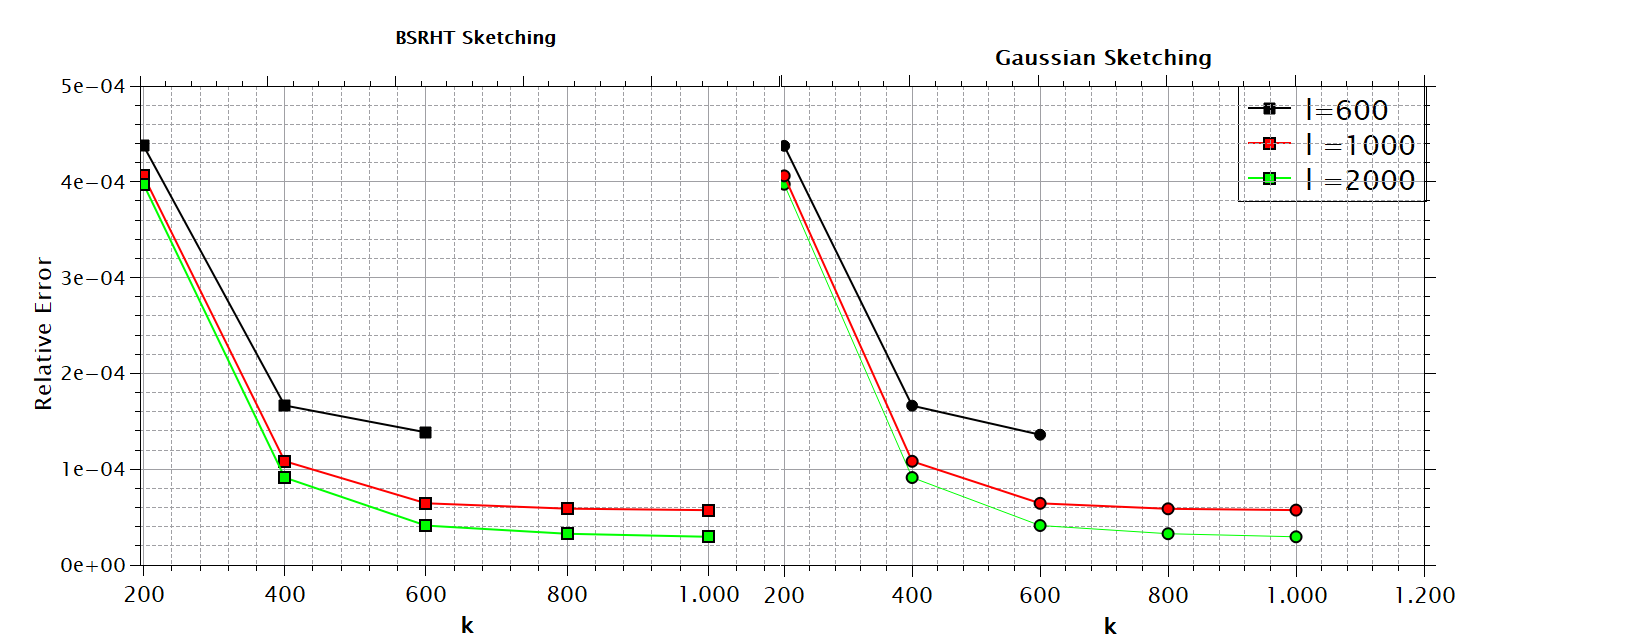
\includegraphics[width=1\textwidth]{../results/plots/accuracy.png}
\end{frame}

\subsection{Performance}
\begin{frame}{Performance}
  \begin{itemize}
    \item Serial and parallel performance evaluated.
    \item Observed $\mathcal{O}(n^2)$ scaling in serial runs.
    \item Strong scaling observed for parallel runs.
  \end{itemize}
  \begin{center}    
    \includegraphics[width=0.45\textwidth]{../results/plots/parallel_runtime.png}
    \includegraphics[width=0.45\textwidth]{../results/plots/parallel_speedup.png}
  \end{center}
\end{frame}

\section{Conclusion}
\begin{frame}{Conclusion}
  \begin{itemize}
    \item Successfully implemented parallel Nystr\"om approximation.
    \item Stable for large matrices.
    \item Improvements: TSQR for QR factorization.
    \begin{itemize}
      \item TSQR for QR factorization.
      \item Compute L by solving $DX =P^{-1}C^T$
    \end{itemize}
  \end{itemize}
\end{frame}

\end{document}
